\documentclass[xetex,mathserif,serif]{beamer}
\usepackage{polyglossia}
\setdefaultlanguage[babelshorthands=true]{russian}
\usepackage{minted}
\usepackage{tabu}
\usepackage{moresize}

\useoutertheme{infolines}

\usepackage{fontspec}
\setmainfont{FreeSans}
\newfontfamily{\russianfonttt}{FreeSans}

\definecolor{links}{HTML}{2A1B81}
\hypersetup{colorlinks,linkcolor=,urlcolor=links}

\setbeamertemplate{blocks}[rounded][shadow=false]

\setbeamercolor*{block title alerted}{fg=red!50!black,bg=red!20}
\setbeamercolor*{block body alerted}{fg=black,bg=red!10}

\tabulinesep=1.2mm

\title{Многопоточное программирование-2}
\subtitle{Высокоуровневая многопоточность}
\author[Юрий Литвинов]{Юрий Литвинов\\\small{\textcolor{gray}{yurii.litvinov@gmail.com}}}
\date{14.09.2018г}

\newcommand{\attribution}[1] {
\vspace{-2mm}\begin{flushright}\begin{scriptsize}\textcolor{gray}{\textcopyright\, #1}\end{scriptsize}\end{flushright}
}

\newcommand{\DownArrow} {
	\hspace{2cm}\begin{LARGE}$\downarrow$\end{LARGE}
}

\begin{document}

	\frame{\titlepage}

	\section{Введение}

	\begin{frame}
		\frametitle{Правда про многопоточность}
		\textbf{Если в вашей программе есть \mintinline{csharp}|new Thread()|, ваша программа уже устарела}
		\begin{itemize}
			\item Проектируйте не в терминах потоков, а в терминах задач, которые могут исполняться параллельно
			\item Доверяйте управление потоками библиотекам
			\item Используйте высокоуровневые языковые средства
			\begin{itemize}
				\item Проще
				\item Надёжнее
				\item Гораздо меньше кода писать
			\end{itemize}
			\item Помните, что внутри всё равно потоки, продумывание синхронизации никто не отменял
			\begin{itemize}
				\item Иногда низкоуровневые потоки внезапно наносят ответный удар
			\end{itemize}
		\end{itemize}
	\end{frame}

	\section{Пул потоков}

	\begin{frame}[fragile]
		\frametitle{Foreground- и Background-потоки}
		\begin{itemize}
			\item Когда все Foreground-потоки завершили работу, рантайм останавливает все Background-потоки и заканчивает работу приложения
			\item Thread по умолчанию создаётся как Foreground
			\begin{itemize}
				\item Способ прострелить себе ногу №1: создать foreground-поток и забыть о нём, приложение будет висеть в списке задач и не завершится
			\end{itemize}
		\end{itemize}
		\vspace{5mm}
		Способ прострелить себе ногу №2: создать background-поток и не дать ему доработать:
		\begin{minted}{csharp}
var t = new Thread(Worker);
t.IsBackground = true;
t.Start();
Console.WriteLine("Returning from Main");
		\end{minted}
	\end{frame}

	\begin{frame}
		\frametitle{Пул потоков}
		\begin{itemize}
			\item Содержит набор заранее созданных потоков, которые могут исполнять задачи
			\item Управляется рантаймом
			\begin{itemize}
				\item Новые потоки создаются при необходимости
				\item Потоки автоматически удаляются, если они долго не используются и потоков больше, чем надо
				\item ``Сколько надо'' рантайм определяет по количеству доступных ядер процессора
			\end{itemize}
			\item Используется в .NET практически повсеместно
			\begin{itemize}
				\item Идеологически многопоточное приложение оперирует не потоками, а задачами и асинхронными операциями
			\end{itemize}
			\item Все потоки из пула --- Background
		\end{itemize}
	\end{frame}

	\begin{frame}[fragile]
		\frametitle{Пример}
		\begin{minted}{csharp}
public static void Main() {
    Console.WriteLine("Главный поток: ставим задачу в очередь");
    ThreadPool.QueueUserWorkItem(ComputeBoundOp, 5);
    Console.WriteLine("Главный поток: занимаемся своими делами...");
    Thread.Sleep(10000);  // Симуляция работы в главном потоке
    Console.WriteLine("Нажмите <Enter>, чтобы закрыть программу...");
    Console.ReadLine();
}

private static void ComputeBoundOp(Object state) {
    Console.WriteLine($"Внутри ComputeBoundOp: state={state}");
    Thread.Sleep(1000);  // Симуляция работы в потоке из пула
}
		\end{minted}
	\end{frame}

	\begin{frame}
		\frametitle{Отмена операций}
		\begin{itemize}
			\item CancellationToken --- отдаётся потоку, он должен сам проверять состояние токена и прерваться, если запрошена отмена
			\begin{itemize}
				\item Может прерваться не мгновенно, проверка возможна только время от времени
				\item Называется ``коллаборативная отмена''
			\end{itemize}
			\item CancellationTokenSource --- возвращает связанный с ним CancellationToken, может выставлять для него флаг отмены, остаётся в основном потоке
		\end{itemize}
	\end{frame}

	\begin{frame}[fragile]
		\frametitle{Пример}
		\begin{small}
			\begin{minted}{csharp}
public static void Main() {
    var cts = new CancellationTokenSource();
    ThreadPool.QueueUserWorkItem(o => Count(cts.Token, 1000));
    Console.ReadLine();
    cts.Cancel();
    Console.ReadLine();
}

private static void Count(CancellationToken token, int countTo) {
    for (int count = 0; count < countTo; count++) {
        if (token.IsCancellationRequested) {
            break;
        }
        Thread.Sleep(200); 
    }
}
			\end{minted}
		\end{small}
	\end{frame}

	\begin{frame}[fragile]
		\frametitle{Полезные вещи CancellationToken}
		\begin{itemize}
			\item \mintinline{csharp}|CancellationToken.None|
			\item \mintinline{csharp}|CancellationToken.Register|:
				\begin{minted}{csharp}
var cts = new CancellationTokenSource();
cts.Token.Register(() => Console.WriteLine("Canceled 1"));
cts.Token.Register(() => Console.WriteLine("Canceled 2"));
				\end{minted}
				\begin{itemize}
					\item Возвращает \mintinline{csharp}|CancellationTokenRegistration|, реализующий \mintinline{csharp}|IDisposable|
				\end{itemize}
		\end{itemize}
	\end{frame}

	\section{Task}

	\begin{frame}[fragile]
		\frametitle{Task}
		\begin{itemize}
			\item Абстракция задачи, которая может быть выполнена в отдельном потоке
			\item Эквивалентные строки кода:
				\begin{minted}{csharp}
ThreadPool.QueueUserWorkItem(ComputeBoundOp, 5);

new Task(ComputeBoundOp, 5).Start();

Task.Run(() => ComputeBoundOp(5));
				\end{minted}
			\item Позволяет ждать окончание задачи и получать результат
			\item Тоже важен для реализации некоторых вещей в C\#, но часто используется и независимо
		\end{itemize}
	\end{frame}

	\begin{frame}[fragile]
		\frametitle{Пример}
		\begin{footnotesize}
			\begin{minted}{csharp}
private static int Sum(int n) {
    int sum = 0;
    for (; n > 0; n--)
        sum += n;
    return sum;
}
...
Task<int> t = new Task<int>(n => Sum((int)n), 1000000000);
t.Start();
// Тут занимаемся своими делами, Sum считается в отдельном потоке из пула
t.Wait();  // t.Result сам делает Wait(), так что тут это только для иллюстрации
Console.WriteLine("Сумма: " + t.Result);
			\end{minted}
		\end{footnotesize}
	\end{frame}

	\begin{frame}[fragile]
		\frametitle{Отмена Task-а}
		\begin{minted}{csharp}
private static int Sum(CancellationToken ct, int n) {
    int sum = 0;
    for (; n > 0; n--) {
        ct.ThrowIfCancellationRequested();
        sum += n;
    }
    return sum;
}
		\end{minted}
		\vspace{3mm}
		Кидает \mintinline{csharp}|OperationCanceledException| в основной поток при обращении к результату (на самом деле, \mintinline{csharp}|AggregateException| с \mintinline{csharp}|OperationCanceledException|)
		\begin{itemize}
			\item Это идеологически правильнее, чем проверять IsCancellationRequested вручную
		\end{itemize}
	\end{frame}

	\begin{frame}[fragile]
		\frametitle{TaskScheduler}
		\begin{itemize}
			\item Класс, позволяющий управлять тем, как Task-и обрабатываются пулом потоков (и пулом потоков ли вообще)
			\begin{itemize}
				\item По умолчанию Task-и ставятся в очередь в пуле потоков
			\end{itemize}
			\item Бывает полезно, например, чтобы задача могла модифицировать элементы GUI
			\begin{itemize}
				\item Это можно делать только из главного потока (который создал GUI)
			\end{itemize}
		\end{itemize}

		\begin{small}
			\begin{minted}{csharp}
Task<int> t = Task.Run(() => Sum(cts.Token, 20000), cts.Token);
t.ContinueWith(task => Text = "Result: " + task.Result,
        CancellationToken.None,
        TaskContinuationOptions.OnlyOnRanToCompletion,
        TaskScheduler.FromCurrentSynchronizationContext());
			\end{minted}
		\end{small}
	\end{frame}

	\section{async/await}

	\begin{frame}
		\frametitle{async/await}
		\begin{columns}
			\begin{column}{0.5\textwidth}
				\begin{itemize}
					\item Task и пул потоков хороши для дорогих по времени операций
					\item Чаще поток ждёт окончания операции ввода-вывода
					\item Блокирующий ввод-вывод ``вешает'' поток, заставляя пул потоков создавать новые
				\end{itemize}
			\end{column}
			\begin{column}{0.5\textwidth}
				\begin{center}
					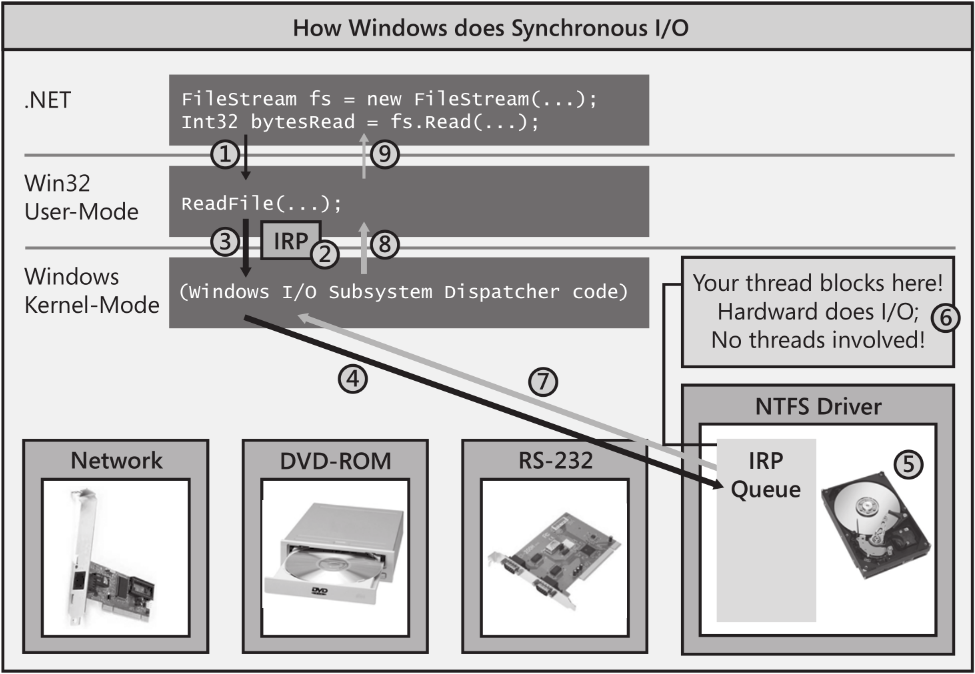
\includegraphics[width=0.9\textwidth]{windowsSynchronousIO.png}
					
					\begin{footnotesize}(Рисунок из Jeffrey Richter. CLR via C\#)\end{footnotesize}
				\end{center}
			\end{column}
		\end{columns}
	\end{frame}

	\begin{frame}
		\frametitle{async/await (2)}
		\begin{columns}
			\begin{column}{0.5\textwidth}
				\begin{itemize}
					\item Асинхронные операции ввода-вывода не блокируют поток, возвращая управление тут же
					\begin{itemize}
						\item Данные, естественно, не готовы
					\end{itemize}
					\item Старая модель в .NET --- \mintinline{csharp}|Begin...()| и \mintinline{csharp}|End...()|
					\begin{itemize}
						\item \mintinline{csharp}|Begin...()| инициирует операцию, принимая колбэк, где можно использовать \mintinline{csharp}|End...()|, чтобы забрать результат
					\end{itemize}
				\end{itemize}
			\end{column}
			\begin{column}{0.5\textwidth}
				\begin{center}
					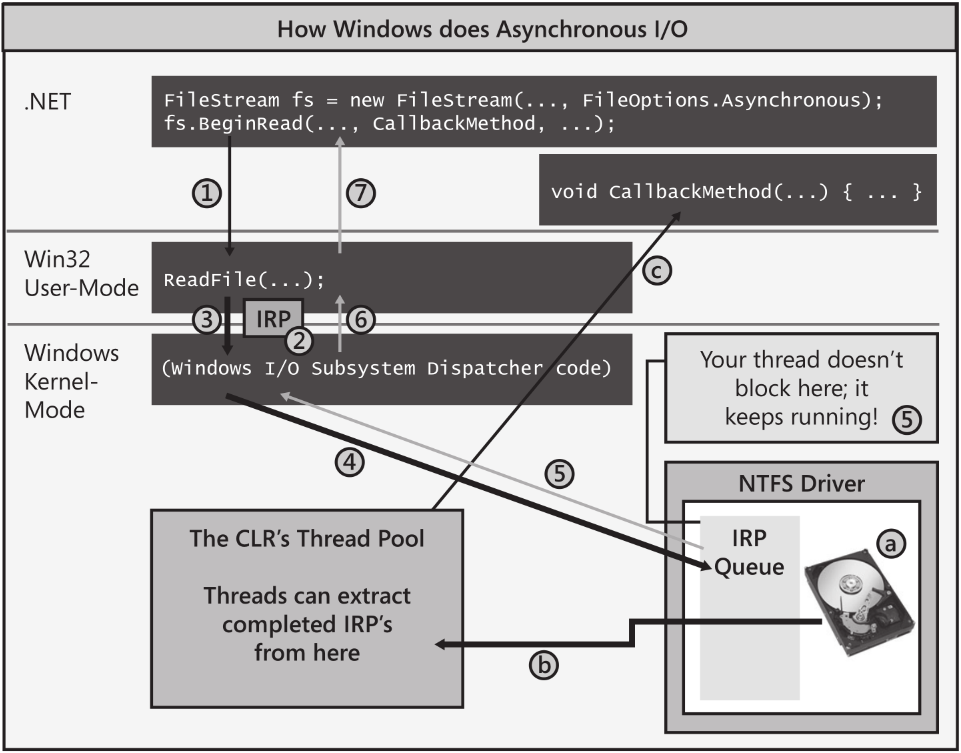
\includegraphics[width=0.9\textwidth]{windowsAsynchronousIO.png}

					\begin{footnotesize}(Рисунок из Jeffrey Richter. CLR via C\#)\end{footnotesize}
				\end{center}
			\end{column}
		\end{columns}
	\end{frame}

	\begin{frame}
		\frametitle{async/await (3)}
		\begin{columns}
			\begin{column}{0.4\textwidth}
				\begin{itemize}
					\item Новая модель: async/await
					\item Требуется поддержка компилятора
					\item Можно понимать как сопрограмму
					\item На самом деле, генерируется конечный автомат
					\begin{itemize}
						\item Запоминает, на каком await сейчас мы находимся
						\item Следит за исключениями
					\end{itemize}
				\end{itemize}
			\end{column}
			\begin{column}{0.6\textwidth}
				\begin{center}
					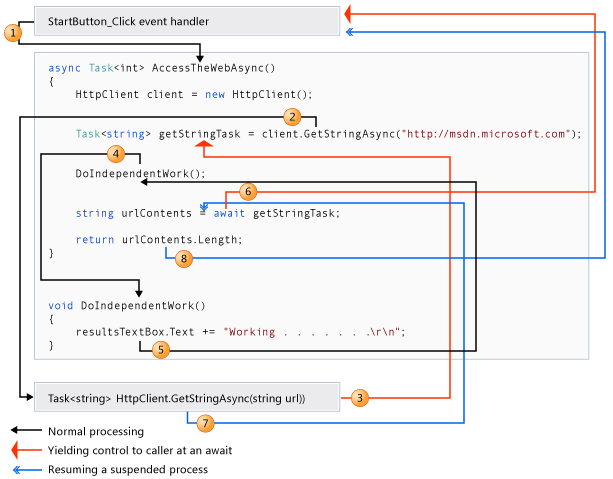
\includegraphics[width=0.9\textwidth]{asyncAwait.png}

					\begin{footnotesize}(Рисунок из \href{https://msdn.microsoft.com/library/hh191443(vs.110).aspx}{MSDN})\end{footnotesize}
				\end{center}
			\end{column}
		\end{columns}
	\end{frame}

	\begin{frame}[fragile]
		\frametitle{Пример}
		\begin{small}
			\begin{minted}{csharp}
private static async Task<int> Method1Async() { ... }
private static async Task<string> Method2Async() { ... }

private static async Task<string> MyMethodAsync(int argument) {
    int local = argument;
    try {
        int result1 = await Method1Async();
        for (int x = 0; x < 3; x++) {
            string result2 = await Method2Async();
        }
    }
    catch (Exception) { Console.WriteLine("Catch"); }
    return "Done";
}
			\end{minted}
		\end{small}
	\end{frame}

	\begin{frame}
		\frametitle{Особенности}
		\begin{itemize}
			\item Может возвращать только \mintinline{csharp}|Task|, \mintinline{csharp}|Task<Result>| или \mintinline{csharp}|void|
			\begin{itemize}
				\item \mintinline{csharp}|void| используется для асинхронных обработчиков событий
			\end{itemize}
			\item Любой Task можно ждать await-ом, любой async можно не ждать
			\begin{itemize}
				\item Вызов Result у результата async-метода заставляет его исполниться синхронно
				\item Если забыть await у асинхронного метода, он вернёт не T, а Task<T>
			\end{itemize}
			\item Работает только с .NET 4.5 и C\# 5
			\begin{itemize}
				\item Microsoft.BCL, если надо поддержать более старый рантайм
			\end{itemize}
		\end{itemize}
	\end{frame}

	\begin{frame}[fragile]
		\frametitle{async и исключения}
		\begin{footnotesize}
			\begin{minted}{csharp}
static async Task ThrowExceptionAsync() {
    await Task.Delay(TimeSpan.FromSeconds(1));
    throw new InvalidOperationException("Всё плохо");
}

static async Task TestAsync() {
    // Исключение не бросается, а сохраняется в Task-е
    Task task = ThrowExceptionAsync();
    try {
        // Исключение бросается при выполнении await (или обращении к Result)
        await task;
    } catch (InvalidOperationException) {
        // Исключение ловится здесь как обычно
    }
}
			\end{minted}
		\end{footnotesize}
	\end{frame}

	\begin{frame}
		\frametitle{Async-методы в стандартной библиотеке}
		\begin{itemize}
			\item \mintinline{csharp}|System.IO.Stream| и потомки: \mintinline{csharp}|ReadAsync|, \mintinline{csharp}|WriteAsync|, \mintinline{csharp}|FlushAsync|, \mintinline{csharp}|CopyToAsync|
			\item \mintinline{csharp}|System.IO.TextReader| и потомки: \mintinline{csharp}|ReadAsync|, \mintinline{csharp}|ReadLineAsync|, \mintinline{csharp}|ReadToEndAsync|, \mintinline{csharp}|ReadBlockAsync|
			\item \mintinline{csharp}|System.IO.TextWriter| и потомки: \mintinline{csharp}|WriteAsync|, \mintinline{csharp}|WriteLineAsync|, \mintinline{csharp}|FlushAsynс|
			\item \mintinline{csharp}|System.Net.Http.HttpClient|: \mintinline{csharp}|GetAsync|, \mintinline{csharp}|GetStreamAsync|, \mintinline{csharp}|GetByteArrayAsync|, \mintinline{csharp}|PostAsync|, \mintinline{csharp}|PutAsync|, \mintinline{csharp}|DeleteAsync| и т.д.
			\item \mintinline{csharp}|System.Net.WebRequest| и потомки: \mintinline{csharp}|GetRequestStreamAsync| и \mintinline{csharp}|GetResponseAsynс|
			\item \mintinline{csharp}|System.Data.SqlClient.SqlCommand|: \mintinline{csharp}|ExecuteDbDataReaderAsync|
		\end{itemize}
	\end{frame}

	\begin{frame}[fragile]
		\frametitle{Ещё один способ прострелить себе ногу}
		\framesubtitle{Вызвать асинхронный метод из GUI-потока и заблокироваться}
		\begin{footnotesize}
			\begin{minted}{csharp}
private sealed class MyWpfWindow : Window {
    public MyWpfWindow() { Title = "WPF Window"; }

    protected override void OnActivated(EventArgs e) {
        string http = GetHttp().Result; // Синхронно вызываемся
        base.OnActivated(e);
    }

    private async Task<String> GetHttp() {
        HttpResponseMessage msg = 
                await new HttpClient().GetAsync("http://google.com/");
        return await msg.Content.ReadAsStringAsync();  // Никогда не дойдём сюда
    }
}
			\end{minted}
		\end{footnotesize}
	\end{frame}

	\begin{frame}[fragile]
		\frametitle{async и Task, полезные вещи}
		\begin{itemize}
			\item Подождать сколько-то миллисекунд:
			\begin{minted}{csharp}
await Task.Delay(delay);
			\end{minted}

			\item Сразу же вернуть результат:
			\begin{minted}{csharp}
// Возвращает Task, который исполняется синхронно
Task.FromResult(13);
			\end{minted}

			\item Подождать несколько Task-ов:
			\begin{minted}{csharp}
int[] results = await Task.WhenAll(task1, task2, task3);
			\end{minted}
		\end{itemize}
	\end{frame}

	\begin{frame}[fragile]
		\frametitle{Task.WhenAny}
		Простой способ организовать таймаут:
		\begin{small}
			\begin{minted}{csharp}
static async Task<string> DownloadStringWithTimeout(string uri)
{
    using (var client = new HttpClient())
    {
        var downloadTask = client.GetStringAsync(uri);
        var timeoutTask = Task.Delay(3000);
        var completedTask = await Task.WhenAny(downloadTask, timeoutTask);
        if (completedTask == timeoutTask)
            return null;
        return await downloadTask;
    }
}
			\end{minted}
		\end{small}
	\end{frame}

	\section{TPL}

	\begin{frame}
		\frametitle{Task Parallel Library}
		\begin{itemize}
			\item Набор классов для выполнения вычислительно сложных параллельных операций (в отличие от async/await, ориентированных на ввод-вывод)
			\begin{itemize}
				\item В стандартной поставке начиная с .NET 4.0
			\end{itemize}
			\item ``Распараллеливание в одну строчку'', берёт на себя управление потоками и ядрами
		\end{itemize}
	\end{frame}

	\begin{frame}[fragile]
		\frametitle{Пример}
		\begin{minted}{csharp}
for (int i = 0; i < 1000; i++) DoWork(i);
		\end{minted}
		\DownArrow
		\begin{minted}{csharp}
Parallel.For(0, 1000, i => DoWork(i));
		\end{minted}

		Или:
		\begin{itemize}
			\item \mintinline{csharp}|Parallel.ForEach(collection, item => DoWork(item));|
			\item 
				\begin{minted}{csharp}
Parallel.Invoke(
    () => Method1(),
    () => Method2(),
    () => Method3());
				\end{minted}
		\end{itemize}
	\end{frame}

	\begin{frame}[fragile]
		\frametitle{Прерывание операции}
		\begin{itemize}
			\item Изнутри:
			\begin{footnotesize}
				\begin{minted}{csharp}
void InvertMatrices(IEnumerable<Matrix> matrices)
{
    Parallel.ForEach(matrices, (matrix, state) => {
        if (!matrix.IsInvertible)
            state.Stop();
        else
            matrix.Invert();
    });
}
				\end{minted}
			\end{footnotesize}

			\item Извне:
			\begin{footnotesize}
				\begin{minted}{csharp}
void RotateMatrices(IEnumerable<Matrix> matrices, float degrees,
    CancellationToken token)
{
    Parallel.ForEach(matrices,
            new ParallelOptions { CancellationToken = token },
            matrix => matrix.Rotate(degrees));
}
				\end{minted}
			\end{footnotesize}
		\end{itemize}
	\end{frame}

	\begin{frame}[fragile]
		\frametitle{Синхронизация нужна}
		\begin{footnotesize}
			\begin{minted}{csharp}
int InvertMatrices(IEnumerable<Matrix> matrices)
{
    object mutex = new object();
    int nonInvertibleCount = 0;
    Parallel.ForEach(matrices, matrix =>
    {
        if (matrix.IsInvertible) {
            matrix.Invert();
        } else {
            // Не лучший способ увеличить счётчик, но как умею :(
            lock (mutex) {
                ++nonInvertibleCount;
            }
        }
    });
    return nonInvertibleCount;
}
			\end{minted}
		\end{footnotesize}
	\end{frame}

	\section{PLINQ}

	\begin{frame}[fragile]
		\frametitle{PLINQ}
		\begin{small}
			\begin{minted}{csharp}
static IEnumerable<int> MultiplyBy2(IEnumerable<int> values)
    => values.AsParallel().Select(item => item * 2);

static IEnumerable<int> MultiplyBy2(IEnumerable<int> values)
    => values.AsParallel().AsOrdered().Select(item => item * 2);

static IEnumerable<int> MultiplyBy2(IEnumerable<int> values)
    => from item in values.AsParallel().AsOrdered() select item * 2;
			\end{minted}
		\end{small}
	\end{frame}

	\begin{frame}
		\frametitle{PLINQ, подробности}
		\begin{itemize}
			\item Реализация LINQ для параллельного исполнения
			\item Работает над любой реализацией IEnumerable и IEnumerable<T>
			\item ``Ленивая'' --- не выполняет операцию, пока её результат не запрошен
			\item Более агрессивно использует ядра, чем TPL
			\item ParallelEnumerable --- класс, предоставляющий почти всю функциональность PLINQ
			\begin{itemize}
				\item Метод-расширение AsParallel() с предыдущего слайда
			\end{itemize}
			\item Может отказаться распараллелить вычисление
		\end{itemize}
	\end{frame}

	\begin{frame}
		\frametitle{Как оно работает}
		\begin{center}
			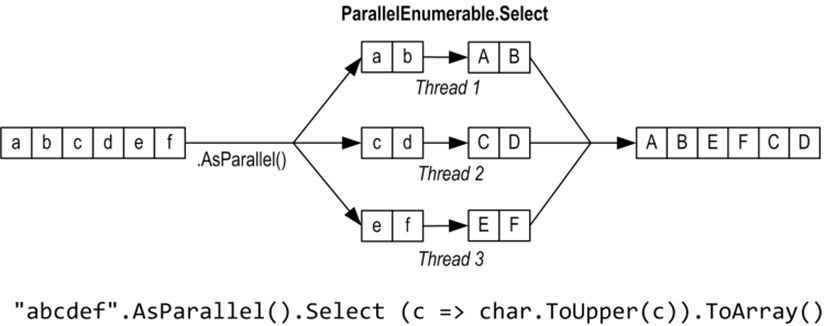
\includegraphics[width=0.9\textwidth]{parallelEnumerable.png}
			\attribution{Joseph Albahari, \url{http://www.albahari.com}}
		\end{center}
	\end{frame}

	\section{Потокобезопасные коллекции}

	\begin{frame}
		\frametitle{Потокобезопасные коллекции}
		\begin{itemize}
			\item Одновременная модификация данных из разных потоков (включая потоки пула, которые используются TPL, PLINQ и т.д.) может привести к гонке
			\item Потокобезопасность --- свойство кода не иметь гонок при обращении из нескольких потоков
			\begin{itemize}
				\item Thread-safe --- возможность вызывать код из нескольких потоков
				\item Reentrant --- возможность вызывать из нескольких потоков, если каждый вызов использует свои данные
				\item Весь thread-safe код reentrant, но не наоборот
			\end{itemize}
			\item Все стандартные коллекции (List<T>, Dictionary<K, V> и т.д.) \textbf{не потокобезопасны}
		\end{itemize}
	\end{frame}

	\begin{frame}
		\frametitle{Немутабельные коллекции}
		Нет изменяемого состояния --- нет гонок
		\begin{itemize}
			\item ImmutableStack<T>
			\item ImmutableQueue<T>
			\item ImmutableList<T>
			\item ImmutableHashSet<T>
			\item ImmutableSortedSet<T>
			\item ImmutableDictionary<K, V>
			\item ImmutableSortedDictionary<K, V>
		\end{itemize}
	\end{frame}

	\begin{frame}[fragile]
		\frametitle{Но как?}
		\begin{minted}{csharp}
var list = ImmutableList<int>.Empty;
list = list.Insert(0, 13);
list = list.Insert(0, 7);

// Пишет "7", затем "13".
foreach (var item in list)
    Console.WriteLine(item);

list = list.RemoveAt(1);
		\end{minted}
	\end{frame}

	\begin{frame}
		\frametitle{А что со скоростью и памятью?}
		\begin{footnotesize}
			\begin{tabu} {| X[0.9 l p] | X[1 l p] | X[1 l p] |}
				\tabucline-
				Операция     & List<T>                & ImmutableList<T>  \\
				\tabucline-
				\everyrow{\tabucline-}
				Add          & амортизированная O(1)  & O(log N)          \\
				Insert       & O(N)                   & O(log N)          \\
				RemoveAt     & O(N)                   & O(log N)          \\
				Item[index]  & O(1)                   & O(log N)          \\
			\end{tabu}
		\end{footnotesize}
		\vspace{5mm}
		Используются сбалансированные двоичные деревья, разделяемые между коллекциями
	\end{frame}

	\begin{frame}[fragile]
		\frametitle{Как это работает}
		\begin{columns}
			\begin{column}{0.6\textwidth}
				\begin{footnotesize}
					\begin{minted}{csharp}
var l1 = ImmutableList.Create<int>();
var l2 = l1.Add(1);
var l3 = l2.Add(2);
var l4 = l3.Add(3);
var l5 = l4.Replace(2, 4);
					\end{minted}
				\end{footnotesize}
			\end{column}
			\begin{column}{0.4\textwidth}
				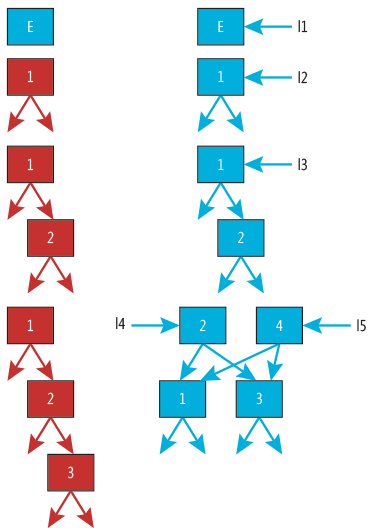
\includegraphics[width=0.9\textwidth]{lists.png}
				\attribution{MSDN}
			\end{column}
		\end{columns}
	\end{frame}

	\begin{frame}
		\frametitle{Потокобезопасные структуры данных}
		Мутабельны, используют примитивы синхронизации для избегания гонок
		\begin{itemize}
			\item Медленны, заметно медленнее немутабельных и ``обычных'' коллекций
			\item Позволяют общаться разным потокам
		\end{itemize}
		Что есть в стандартной библиотеке:
		\begin{itemize}
			\item ConcurrentDictionary<K, V>
			\item BlockingCollection<T>
			\item ConcurrentBag<T>
			\item ConcurrentQueue<T>
			\item ConcurrentStack<T>
		\end{itemize}
	\end{frame}

	\begin{frame}[fragile]
		\frametitle{Пример}
		\begin{scriptsize}
			\begin{minted}{csharp}
var cq = new ConcurrentQueue<int>();

for (int i = 0; i < 10000; i++) 
    cq.Enqueue(i);

if (!cq.TryPeek(out int result))
    Console.WriteLine("С TryPeek тут всё должно было быть ок");
else if (result != 0)
    Console.WriteLine($"Ожидалось 0, получили {result}");

int outerSum = 0;
Action action = () => {
    int localSum = 0;
    while (cq.TryDequeue(out int localValue)) 
        localSum += localValue;
    // Более правильный способ прибавлять, о котором потом
    Interlocked.Add(ref outerSum, localSum);
};

Parallel.Invoke(action, action, action, action);

Console.WriteLine($"outerSum = {outerSum}, should be 49995000");
			\end{minted}
		\end{scriptsize}
	\end{frame}

	\section{Заключение}

	\begin{frame}
		\frametitle{Литература}
		\begin{columns}
			\begin{column}{0.6\textwidth}
				Stephen Cleary, Concurrency in C\# Cookbook, O'Reilly Media, 2014. 207PP.

				\textcolor{gray}{Многие примеры взяты оттуда}
			\end{column}
			\begin{column}{0.4\textwidth}
				\begin{center}
					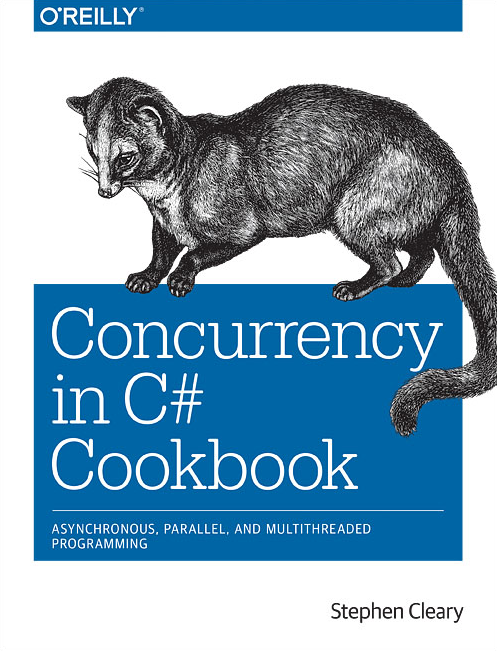
\includegraphics[width=0.6\textwidth]{concurrencyCookbookCover.png}
				\end{center}
			\end{column}
		\end{columns}
	\end{frame}

\end{document}
